\section{Конструкторский раздел}

В данном разделе будут рассмотрены основные методы, которые были использованы
при разработке программного обеспечения.

\subsection{Алгоритм работы приложения}

Схема алгоритмa работы приложения представлена на рисунке \ref{fig:main_diagram}.
Рассмотрим каждый этап более подробно.

\begin{figure}[p]
    \centering
    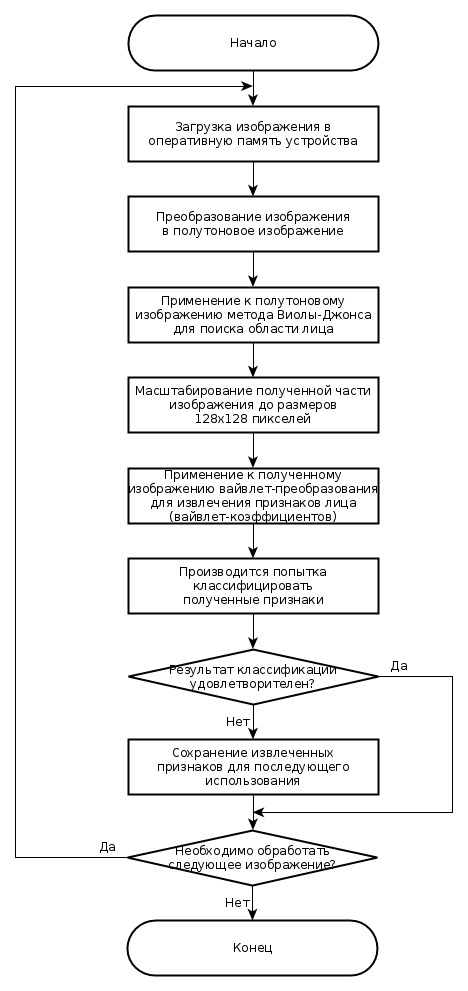
\includegraphics[height=.95\textheight]{main_diagram.png}
    \caption{Cхема алгоритма работы приложения}
    \label{fig:main_diagram}
\end{figure}

\subsection{Обнаружение лица на фотоснимке}

В качестве метода обнаружения лица на фотоснимке был выбран метод Виолы-Джонса.
Данный метод был выбран за его репрезентативние возможности, независимость от условий
освещенности, высокие показатели обнаружения и высокую скорость работы.

\subsubsection{Обучение классификатора в методе Виолы-Джонса}

В контексте алгоритма, имеется множество объектов (изображений), разделённых некоторым образом на классы. Задано конечное
множество изображений, для которых известно, к какому классу они относятся (к примеру, это может быть класс <<фронтальное положение
носа>>). Это множество называется \textit{обучающей выборкой}. Классовая принадлежность остальных объектов не известна. Требуется построить
алгоритм, способный классифицировать произвольный объект из исходного множества \cite{viola_jones}.

\textit{Классифицировать объект}~-- значит, указать номер (или наименование класса), к которому относится данный объект.

\textit{Классификация объекта}~-- номер или наименование класса, выдаваемые алгоритмом классификации в результате его применения к данному
конкретному объекту.

\textit{Классификатор}(classifier)~-- в задачах классификации это аппроксимирующая функция, выносящая решение, к какому именно классу данный
объект принадлежит.

\textit{Обучающая выборка}~-- конечное число данных.

В машинном обучении задача классификации относится к разделу обучения с учителем когда классы поделены. Распознавание образов по
сути своей и есть классификация изображений и сигналов. В случае алгоритма Виолы-Джонса для идентификации и распознавания лица
классификация является двухклассовой.

Постановка классификации выглядит следующим образом:

Есть $X$~-- множество, в котором хранится описание объектов, $Y$~-- конечное множество номеров, принадлежащих классам. Между ними есть
зависимость~-- отображение $Y*: X \Rightarrow Y$. Обучающая выборка представлена $Xm = \lbrace(x_1,y_1), \dots, (x_m,y_m)\rbrace$.
Конструируется функция $f$ от
вектора признаков $X$, которая выдает ответ для любого возможного наблюдения $X$ и способна классифицировать объект $x\in X$. Данное
простое правило должно хорошо работать и на новых данных.

\subsubsection{Применяемый в алгоритме бустинг}

Для решения проблемы данного, столь сложного обучения существует технология бустинга. 

Бустинг~-- комплекс методов, способствующих повышению точности аналитических моделей. Эффективная модель, допускающая мало ошибок
классификации, называется <<сильной>>. <<Слабая>> же, напротив, не позволяет надежно разделять классы или давать точные предсказания,
делает в работе большое количество ошибок. Поэтому бустинг (от англ. \textit{boosting}~-- повышение, усиление, улучшение) означает дословно
<<усиление>> <<слабых>> моделей~\cite{viola_jones_2}~-- это процедура последовательного построения композиции алгоритмов машинного обучения, когда
каждый следующий алгоритм стремится компенсировать недостатки композиции всех предыдущих алгоритмов.

В основе такой идеи лежит построение цепочки (ансамбля) классификаторов \cite{viola_jones_2}, который называется каскадом, каждый из которых
(кроме первого) обучается на ошибках предыдущего. Например, один из первых алгоритмов бустинга \textit{Boost1} использовал каскад из 3-х
моделей, первая из которых обучалась на всем наборе данных, вторая~-- на выборке примеров, в половине из которых первая дала
правильные ответы, а третья~-- на примерах, где <<ответы>> первых двух разошлись. Таким образом, имеет место последовательная
обработка примеров каскадом классификаторов, причем так, что задача для каждого последующего становится труднее. Результат
определяется путем простого голосования: пример относится к тому классу, который выдан большинством моделей каскада.

Бустинг представляет собой жадный алгоритм построения композиции алгоритмов (\textit{greedy algorithm})~-- это алгоритм, который на каждом
шаге делает локально наилучший выбор в надежде, что итоговое решение будет оптимальным. Бустинг над решающими деревьями считается
одним из наиболее эффективных методов с точки зрения качества классификации. Во многих экспериментах наблюдалось практически
неограниченное уменьшение частоты ошибок на независимой тестовой выборке по мере наращивания композиции. Более того, качество на
тестовой выборке часто продолжало улучшаться даже после достижения безошибочного распознавания всей обучающей выборки. Это
перевернуло существовавшие долгое время представления о том, что для повышения обобщающей способности необходимо ограничивать
сложность алгоритмов. На примере бустинга стало понятно, что хорошим качеством могут обладать сколь угодно сложные композиции,
если их правильно настраивать \cite{viola_jones_2}.

Математически бустинг объясняется следующим образом.

Наряду с множествами $X$ и $Y$ вводится вспомогательное множество $R$, называемое \textit{пространством оценок}. Рассматриваются алгоритмы,
имеющие вид суперпозиции $a(x) = C(b(x))$, где функция $b: X \rightarrow R$ называется \textit{алгоритмическим оператором},
функция $C: R \rightarrow Y$~-- \textit{решающим правилом}.

Многие алгоритмы классификации имеют именно такую структуру: сначала вычисляются оценки принадлежности объекта классам, затем
решающее правило переводит эти оценки в номер класса. Значение оценки, как правило, характеризует степень уверенности
классификации.

\textit{Алгоритмическая композиция}~-- алгоритм $a: X \rightarrow Y$ \cite{viola_jones_2} вида:
\begin{equation}
a(x) = C(F(b_1(x), \dots, b_T(x))),\ x\in X,
\end{equation}
составленный из алгоритмических операторов $b_t: X \rightarrow R,\ t = \overline{1,\dots,T}$,
корректирующий операции $ F: R^T\rightarrow R $ и решающего правила $ C: R \rightarrow Y$.

\textit{Базовыми алгоритмами} обозначаются функции $a_t(x) = C(b_t(x)) $, а при фиксированном решающем правиле $C$~-- и сами
операторы $b_t(x)$ \cite{viola_jones_2}.

Суперпозиции вида $F(b_1, \dots, b_T)$ являются отображениями $X \rightarrow R$, то есть, опять же, алгоритмическими операторами.

В задачах классификации на два непересекающихся класса в качестве пространства оценок обычно используется множество действительных
чисел. Решающие правила могут иметь настраиваемые параметры. Так, в алгоритме Виолы-Джонса используется \textit{пороговое решающее
правило}, где, как правило, сначала строится оператор при нулевом значении, а затем подбирается значение оптимальное. Процесс
последовательного обучения базовых алгоритмов применяется, чаще всего при построении композиций \cite{viola_jones_2}.

\textit{Критерии останова} могут использоваться различные, в зависимости от специфики задачи, возможно также совместное применение
нескольких критериев:
\begin{itemize}
    \item построено заданное количество базовых алгоритмов $T$;
    \item достигнута заданная точность на обучающей выборке;
    \item достигнутую точность на контрольной выборке не удаётся улучшить на протяжении последних нескольких шагов при определенном
        параметре алгоритма.
\end{itemize}

Развитием данного подхода явилась разработка более совершенного семейства алгоритмов бустинга AdaBoost (\textit{adaptive boosting}~--
адаптированное улучшение), который может использовать произвольное число классификаторов и производить обучение на одном наборе
примеров, поочередно применяя их на различных шагах.

Рассматривается задача классификации на два класса, $Y = \lbrace  -1,+1 \rbrace$. К примеру, базовые алгоритмы также возвращают только два ответа
$-1$ и $+1$, и решающее правило фиксировано: $C(b) = sign(b)$. Искомая алгоритмическая композиция имеет вид \cite{viola_jones_2}:
\begin{equation}
    a(x) = C(F(b_1(x), \dots, b_T(x))) = sign(\sum_{t=1}^Ta_tb_t(x)),\ x\in X
\end{equation}

\textit{Функционал качества композиции} $Q_T$ определяется как число ошибок, допускаемых алгоритмом на обучающей выборке:
\begin{equation}
    Q(b, \overline{W}^l) = Q_T = \sum_{i=1}^l(y_i\sum_{t=1}^Ta_tb_t(x_i))<0,
\end{equation}
где $\overline{W}^l = (w_1,\dots,w_l)$~-- вектор весов объектов.

Общий алгоритм адаптивного усиления, AdaBoost, выглядит следующим образом~\cite{viola_jones_2}.

Дано:
\begin{itemize}
    \item $ Y = \lbrace -1,+1 \rbrace $;
    \item $b_1(x), \dots, b_T(x) $ возвращают $-1$ и $+1$;
    \item $X^l$~-- обучающая выборка.
\end{itemize}

Решение:
\begin{enumerate}
    \item Инициализация весов объектов: $w_i=\frac{1}{l},\ i=1,\dots,l$;
    \item Для всех $ t = \overline{1, \dots, T}$, пока не выполнен критерий останова:
        \begin{enumerate}
            \item $ b_t = arg\,min_b(Q(b, \overline{W}^l)) $;
            \item $ a_t = \frac{1}{2\ln1} - \frac{1 - Q(b_t, \overline{W}^l)}{Q(b_t, \overline{W}^l)} $;
        \end{enumerate}
    \item Пересчёт весов объектов: $$ w_i = w_i e^{-a_ty_ib_t(x_i)},\ i=\overline{1,\dots,l}; $$
    \item Нормировка весов объектов: $$ w_0 = \sum_{j=1}^lw_j;\ w_i=\frac{w_i}{w_0},\ i=\overline{1,\dots,l}. $$
\end{enumerate}

Плюсы AdaBoost:
\begin{itemize}
    \item хорошая обобщающая способность. В реальных задачах практически всегда строятся композиции, превосходящие по качеству базовые
        алгоритмы. Обобщающая способность может улучшаться по мере увеличения числа базовых алгоритмов;
    \item простота реализации;
    \item собственные накладные расходы бустинга невелики. Время построения композиции практически полностью определяется временем обучения
        базовых алгоритмов;
    \item возможность идентифицировать объекты, являющиеся шумовыми выбросами. Это наиболее <<трудные>> объекты $x_i$, для которых в процессе
        наращивания композиции веса $w_i$ принимают наибольшие значения.
\end{itemize}

Минусы AdaBoost:
\begin{itemize}
    \item бывает переобучение при наличии значительного уровня шума в данных. Экспоненциальная функция потерь слишком сильно увеличивает
        веса <<наиболее трудных>> объектов, на которых ошибаются многие базовые алгоритмы. Однако именно эти объекты чаще всего оказываются
        шумовыми выбросами. В результате AdaBoost начинает настраиваться на шум, что ведёт к переобучению. Проблема решается путём
        удаления выбросов или применения менее <<агрессивных>> функций потерь. В частности, применяется алгоритм GentleBoost;
    \item AdaBoost требует достаточно длинных обучающих выборок. Другие методы линейной коррекции, в частности, бэггинг, способны строить
        алгоритмы сопоставимого качества по меньшим выборкам данных;
    \item бывает построение неоптимального набора базовых алгоритмов. Для улучшения композиции можно периодически возвращаться к ранее
        построенным алгоритмам и обучать их заново;
    \item бустинг может приводить к построению громоздких композиций, состоящих из сотен алгоритмов. Такие композиции исключают возможность
        содержательной интерпретации, требуют больших объёмов памяти для хранения базовых алгоритмов и существенных временных затрат на
        вычисление классификаций.
\end{itemize}

В наши дни подход усиления простых классификаторов является популярным и, вероятно, наиболее эффективным методом классификации за
счёт высокой скорости и эффективности работы и относительной простоты реализации.

\subsubsection{Принципы решающего дерева в разрабатываемом алгоритме}

\textit{Дерево принятия решений}~-- это дерево, в листьях которого стоят значения целевой функции, а в остальных узлах~-- условия перехода (к
примеру, на Лице есть Улыбка), определяющие по какому из ребер идти. Если для данного наблюдения условие равно истине то
осуществляется переход по левому ребру, если же ложь~-- по правому\cite{viola_jones_2}.

Достоинствами таких решающих деревьев являются наглядность, легкость работы с ними, быстродействие. Также, они легко применяются
для задач с множеством классов.

\subsubsection{Каскадная модель разрабатываемого алгоритма}

Алгоритм бустинга для поиска лиц следующий:
\begin{enumerate}
    \item Определение слабых классификаторов по прямоугольным признакам;
    \item  Для каждого перемещения сканирующего окна вычисляется прямоугольный признак на каждом примере;
    \item Выбирается наиболее подходящий порог для каждого признака;
    \item Отбираются лучшие признаки и лучший подходящий порог;
    \item Перевзвешивается выборка.
\end{enumerate}

\textit{Каскадная модель сильных классификаторов}~-- это дерево принятия решений, где каждый узел дерева построен таким
образом, чтобы детектировать почти все интересующие образы и отклонять регионы, не являющиеся образами. Помимо этого, узлы дерева
размещены таким образом, что чем ближе узел находится к корню дерева, тем из меньшего количества примитивов он состоит и тем самым
требует меньшего времени на принятие решения. Данный вид каскадной модели хорошо подходит для обработки изображений, на которых
общее количество детектируемых образов мало~\cite{viola_jones_2}.

В этом случае метод может быстрее принять решение о том, что данный регион не содержит образ, и перейти к следующему.
Пример модели сильных классификаторов представлен на рисунке \ref{fig:adaboost}.

\begin{figure}
    \centering
    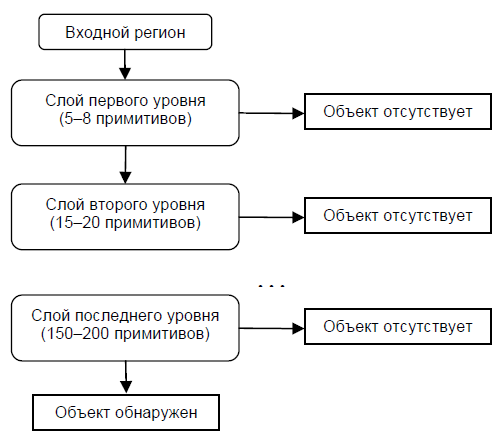
\includegraphics[height=.3\textheight]{145644c4.png}
    \caption{Пример каскадной модели сильных классификаторов}
    \label{fig:adaboost}
\end{figure}

Сложность обучения таких каскадов равна $О(xyz)$, где применяется $x$ этапов, $y$ примеров и $z$ признаков.

Далее, каскад применяется к изображению:
\begin{enumerate}
    \item Работа с <<простыми>> классификаторами~-- при этом отбрасывается часть <<отрицательных>> окон;
    \item Положительное значение первого классификатора запускает второй, более приспособленный и так далее;
    \item Отрицательное значение классификатора на любом этапе приводит к немедленному переходу к следующему сканирующему окну,
        старое окно отбрасывается;
    \item Цепочка классификаторов становится более сложной, поэтому ошибок становится намного меньше.
\end{enumerate}

Для тренировки такого каскада потребуются следующие действия:
\begin{enumerate}
    \item Задаются значения уровня ошибок для каждого этапа~-- они называются \textit{detection} и \textit{false positive
        rates}~-- надо чтобы уровень detection был высок, а уровень false positive rates низок;
    \item Добавляются признаки до тех пор, пока параметры вычисляемого этапа не достигнут поставленного уровня, тут возможны такие
        вспомогательные этапы, как:
        \begin{enumerate}
            \item тестирование дополнительного маленького тренировочного набора;
            \item порог AdaBoost умышленно понижается с целью найти больше объектов, но в связи с этим возможно большее число
                неточных определений объектов;
        \end{enumerate}
    \item Если false positive rates остается высоким, то добавляется следующий этап или слой;
    \item Ложные обнаружения в текущем этапе используются как отрицательные уже на следующем слое или этапе.
\end{enumerate}

\subsubsection{Алгоритм скользящего окна}

В ходе обнаружения лица на изображения, алгоритм Виолы-Джонса использует
метод скользящего окна, который позволяет перебрать все возможные варианы местонахождения
искомого объекта. На входе алгоритму передается изображение размера $ width \times height $.

Алгоритм представлен схемой, изображенной на рисунке \ref{fig:lala_window}.

\begin{figure}[p]
    \centering
    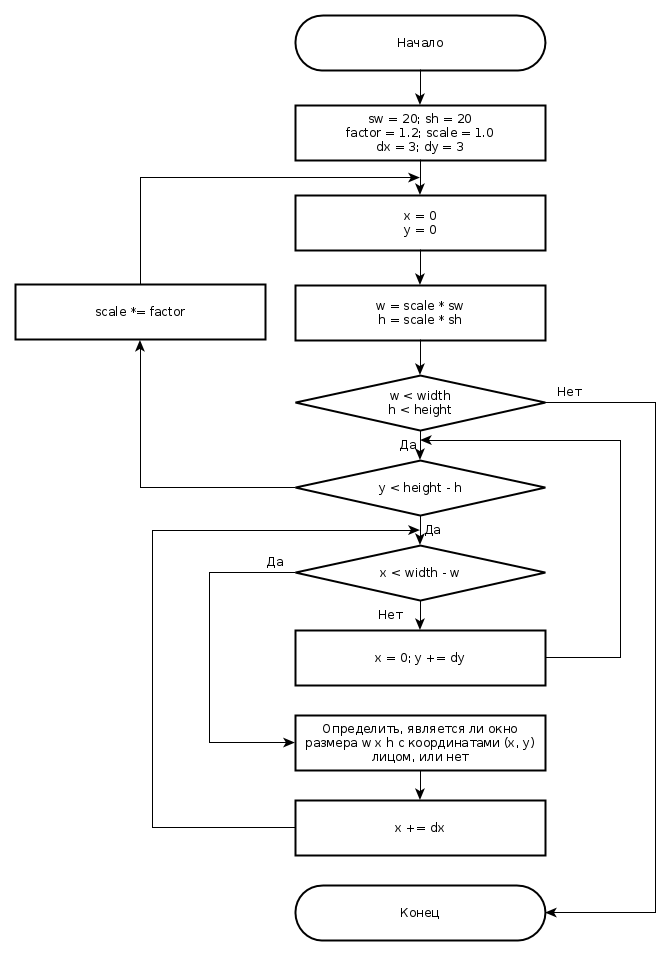
\includegraphics[width=0.8\textwidth]{lala_window.png}
    \caption{Схема алгоритма скользящего окна}
    \label{fig:lala_window}
\end{figure}

\subsubsection{Алгоритм Виолы-Джонса}

Ранее были рассмотрены основные моменты, которые должны быть использованы в работе алгоритма
Виолы-Джонса. Рассмотрим теперь алгоритм работы метода Виолы-Джонса в полном объеме.

На вход алгоритму подается изображение в градиентах серого. Результатом работы алгоритма
является квадратная область, которая характеризует местонахождение лица на фотоснимке.

Распознавание в этом методе осуществляется по <<прецедентам>> \cite{viola_jones_2}. В помощью
<<обучающей выборки>> строится набор <<сильных классификаторов>>, каждый из которых
для квадратного окна говорит: <<предположительно, в окне~-- лицо>>, или~--
<<определенно, не лицо>>. Таким образом, для того, чтобы алгоритм признал
картинку в окне за лицо, необходимо, чтобы все <<сильные классификаторы>> (stages)
ответили: <<да, лицо предположительно есть>>. Если хотя бы один из них отверг
окно (сказал, что <<лица определенно нет>>), то алгоритм сразу же отвергает
данное окно, другие <<сильные классификаторы>> не использует, и переходит
к следующему окну.

Опишем работу алгоритма псевдокодом:
\begin{verbatim}
failed = 0
цикл по stages
    sum_stage = 0.0
    цикл по features
        sum_feature = 0.0
        цикл по rects
            sum_feature += Sum(x,y,w,h) * rect.weight
        конец цикла
        если sum_feature < feature_threshold, то
            sum_stage += feature.left_val
        иначе
            sum_stage += feature.right_val
    конец цикла
    если sum_stage < stage_threshold, то
        failed = 1
        break
конец цикла
вернуть failed
\end{verbatim}

На вход алгоритму подается часть изображения~-- скользящее окно.
Результатом работы алгоритма является число: 1~-- если на выбранной позиции скользящего окна расположено лицо и 0 иначе.
При этом в алгоритме выше не учитывается масштабирование рассматриваемых прямоугольных признаков
до размеров выбранного окна.

Для выбранной позиции скользящего окна, перебираются все <<сильные
классификаторы>> (\textit{stages}) и <<хааро-подобные функции>> (\textit{features}). Для каждой
\textit{feature} считается сумма интенсивностей пикселов с определенным весовым
коэффициентом по <<белой>> области \textit{feature} (см. рис. \ref{fig:haar}), и вычитается сумма
по <<тёмной>> области, с другим весовым коэффициентом. Полученная сумма
умножается на величину \textit{inv}, и сравнивается
с порогом <<feature threshold>>, умноженным на величину \textit{stddev}. Если первое~--
меньше второго, то к сумме по \textit{stage} (<<сильному классификатору>>) добавляется
величина \textit{left\_val} данного \textit{feature}, иначе~-- добавляется величина \textit{right\_val}.

\subsection{Конвертация изображения}

В качестве метода для представления
изображения, как информации для последующей классификации, был выбран метод
вайвлет-преобразований. Данный метод был выбран за его репрезентативные
возможности, независимость от условий освещенности, приемлемые показатели
распознавания, высокую скорость работы, простоту реализации и возможность
распараллеливания вычислений.

На данном шаге алгоритма на вход поступает изображение лица в формате градаций серого.
Далее к изображению применяется двумерное преобразование Добеши D4~\cite{vaivlet_1}.

\subsection{Классификация} В качестве классификатора была выбрана нейронная
сеть. Нейронная сеть представляет собой упрощенную математическую модель нервной
системы живых существ, в частности, головной мозг человека. Была выбрана сеть с
прямым распространением сигнала. Определение сети и алгоритм её обучения будут
представлены согласно \cite{merkov}.


Нейронная сеть прямого распространения - это связный ориентированный
ациклический граф с множеством вершин $V = \{v_1,\dots,v_S\}$ (рецепторов и
нейронов) и ребер (синапсов) $E = {e_1,\dots,e_T}$, снабженный следующей
дополнительной структурой:
\begin{enumerate}
\item множества вершин-истоков (рецепторов) $V_{in}$ и вершин-стоков (выходных
нейронов) $V_{out}$ нейронной сети (непустые, как у всякого связного
ориентированного ациклического графа) упорядочены;
\item каждому ребру $e$ приписан параметр $w_e \in \Re$ и функция $f_e:\Re^2 \to
\Re$, называемая функцией проводимости ребра (синапса);
\item каждой вершине $v \in V \ V_{in}$ приписан параметр $w_v \in \Re$ и
функция $g_v:\Re^2 \to \Re$, называемая функцией активации вершины (нейрона).
\end{enumerate}

Упорядоченные множества $V_{in} = (v_{in}^1,\dots,v_{in}^d)$ и $V_{out} =
(v_{out}^1,\dots,v_{out}^q$ содержат $d$ и $q$ вершин, соответственно. Нейронная
сеть вычисляет вектор-функции $f : \Re^d \to \Re^q$ , зависящие также от
параметров всех вершин и ребер сети. Для вычисления значения $y = f (x)$ на
вершинах и ребрах сети определяется вспомогательная вещественнозначная функция u
(потенциал), зависящая от вектор-аргумента $x$ и параметров сети $w$, причем
потенциал $u(e)$ каждого ребра e равен потенциалу $u(v)$ вершины $v$, из которой
это ребро выходит $(e \in V_{out})$. Потенциал определяется индуктивно:
\begin{enumerate}
\item потенциал j-го источка $v_{in}^j$ равен j-му аргументу $x^j$,
т.е. $u(v_{in}^j = x^j$;
\item для каждой вершины $v$, для всех входящих ребер которой входные потенциалы
уже определены, вычисляется активирующая сумма
\[ s(v) = \sum_{e \in v_{in}} h_e(w_e,u(e)) \] и потенциал
\[ u(v) = g_v(w_v,s(v)) .\]
\end{enumerate}

Связность и ацикличность сети гарантируют корректное вычисление потенциала
каждой вершины. Результатом вычисления является вектор-потенциал $y =
(y^1,\dots,y^q) = (u(v_{out}^1),\dots,u(v_{out}^q))$ вершин-стоков.


Вектор $w$, составленный из всех чисел $w_e$ и $w_v$ , является параметром
сети. Обучение нейронной сети заключается в подборе такого значения $w$, чтобы
выходной вектор $y$, являющийся функцией $y = f(x) = F(w, x)$ от параметра и
входного вектора $x$, был похож на то, чему сеть пытаются научить. Наоборот,
функции $h_e$ и $g_v$ и сам ориентированный граф остаются неизменными.


Для простоты и удобства реализации нейронной сети обычно полагают ее состоящей
из нейронов нескольких (немногих) разновидностей, регулярным образом соединенных
друг с другом. Чаще всего множество $V$ всех нейронов сети предполагаются
разбитым на пронумерованные слои $V_0 = V_{in}, V_1,\dots,V_L = V_{out}$, так
что
\begin{enumerate}
\item каждое ребро, входящее в нейрон некоторого i-го слоя, выходит из некторого
нейрона (i-1)-го слоя;
\item для каждого слоя функции активации $g_v$ всех нейронов этого слоя
совпадают; совпадают и функции проводимости $h_e$ всех входящих в них ребер.
\end{enumerate}

Такая нейронная сеть называется L-слойной. Послойная градуировка автоматически
обеспечивает ацикличность сетей. В практически применяемых нейронных сетях
послойная структура может быть более сложной и не вполне регулярной.


Наиболее типичными для многослойных сетей являются следующие функции
проводимости ребер и активации нейронов:
\begin{enumerate}
\item $h_e(w_e,u) = w_eu$, а $g_v(w_v,s) = th(s - w_v)$ (гиперболический тангенс
разности), $g_v(w_v,s) = \sigma(s-w_v)$ (логическая функция от разности), или
какое-нибудь другое гладкое монотонно возрастающее приближение ступенчатой
функции;
\item $h_e(w_e,u) = (u - w_e)^2$, а $g_v(w_v,s) = e^{-s/2w_v}$ или какое -нибудь
другое гладкое приближение дельта-функции.
\end{enumerate} Функция активации выходных нейронов (нейронов последнего слоя)
обычно определяется задачей, для решения которой нейронная сеть предназначена.


Искусственные нейронные сети могут применяться для вычисления функций как от
дискретных, так и от непрерывных признаков. В последнем случае для устойчивости
сети к ошибкам измерения входных векторов необходима непрерывность функций $h_e$
и $g_v$ , а для обучения сети градиентными методами — еще и их
дифференцируемость. В дальнейшем функции $h_e$ и $g_v$ предполагаются гладкими.


Количество L слоев в практически применяемых нейронных сетях на удивление мало:
чаще всего встречаются трехслойные сети, иногда даже двухслойные. И наоборот, в
одном и том же распознавании иногда участвуют несколько различных сетей, как-то
соединенных друг с другом, но обучаемых раздельно. Сеть может и не иметь никакой
регулярной многослойной структуры.


Количество $d$ входов искусственной сети и количество $q$ ее выходных нейронов
определяются решаемой задачей и обычно не очень велики. $d$ равно размерности
пространства признаков (обычно десятки или сотни), а $q$ меняется от 1
(регрессия) до сотен (многоклассовая классификация). Наоборот, число остальных
нейронов, называемых скрытыми, бывает порядка тысяч и десятков тысяч, а число
ребер доходит до миллионов, хотя это несравнимо меньше, чем в естественной
нейронной сети. В искусственных нейронных сетях, как и в мозгу, все вычисления
могут происходить параллельно, и тем самым, очень быстро. В реальности нейронные
сети моделируются на обычных последовательных компьютерах и работают не слишком
быстро, а главное, медленно обучаются, поэтому на количестве вершин и ребер сети
приходится экономить. Появляющиеся время от времени аппаратные реализации
нейронных сетей (нейрокомпьютеры) позволяют несколько увеличить размеры
пригодных для обучения сетей.


Создание нейронной сети для решения какой-либо задачи состоит из двух этапов:
построение сети, т.е. ациклического ориентированного графа и функций
проводимости и активации, и подбор ее параметров w. Первый этап — очень
эвристический и существенно зависящий от конкретной решаемой задачи и объема
доступных обучающих данных, и как правило требует многочисленных
экспериментов. Для второго этапа — обучения — применяются довольно универсальные
методы.


Типичный распознающий перцептрон — трехслойный. Нейроны первого скрытого слоя
разбиты на несколько групп: внутри каждой группы нейроны одинаковы и соединены
не со всеми входами сети, а только с каким-то их подмножеством, своим для каждой
группы. Это разбиение на группы производится вручную исходя из специфики
задачи. Например, при распознавании растровых изображений каждый нейрон первого
слоя может иметь свое небольшое “поле зрения”, т.е. быть соединенным с
рецепторами, измеряющими яркость изображения в некотором количестве (нескольких
десятках) смежных точек. Поля зрения разных нейронов одной группы сдвинуты друг
относительно друга (обычно поля зрения “соседних” нейронов перекрываются), а
нейроны разных групп имеют разные по размеру и по форме поля зрения. Нейроны
второго скрытого слоя более-менее одинаковы, но каждый нейрон соединен со
случайным не слишком большим подмножеством нейронов первого слоя. Каждый нейрон
третьего слоя (выходного) соединен со всеми нейронами второго слоя.

\subsubsection{Обучение многослойного перцептрона: метод обратного распространения ошибки (error back-propagation).}
Обучение перцептрона, вычисляющего функцию F(w,x) --- это поиск вектора весой и
смещений w, минимзирующего регуляризованную суммарную ошибку
\[ E_T(w) = \phi(w) + \sum_{i=1}^NE(F(w,x_i),y_i) \]
на некотором обучающем наборе $T = ((x_1,y_1),\dots,(x_N,y_N))$. Обучение чаще
всего производится методом градиентного спуска и комбинированием его с другими
методами. Для его применимости функции активации всех нейронов и функции ошибки
$E$ и регуляризации $\phi$ должны быть дифференциируемы. Вычисление градиента не
совсем просто из-за огромной размерности параметра $w$ и отсутствия явных формул
для производных функции $F$ по $w$.


Замечательно то, что этот огромной размерности градиент ошибки по параметру для
нейронной сети можно вычислять красиво и быстро — за время того же порядка, что
и время работы сети — с помощью другой (двойственной) нейронной сети,
получающейся из исходной обращением направлений ребер. На этом основании
градиентный спуск для нейронных сетей обычно называется не просто градиентным
спуском, а методом обратного распространения ошибки. Хотя строго говоря, метод
обратного распространения — это всего лишь способ вычисления градиента ошибки, и
даже не обязательно ошибки, а любой функции от выхода нейронной
сети. Конфигурация двойственной сети однозначно определена конфигурацией
исходной сети, а веса и функции активации зависят от весов ребер исходной сети и
набора значений $\{u(v)\}$ потенциалов нейронов. А именно,
\begin{enumerate}
\item нейронами $\breve{v}\dots$ двойственной сети являются все скрытые нейроны
и входы $v\dots$ исходной сети;
\item входами $\breve{v}_L^1,\dots,\breve{v}_L^q$ двойственной сети являются
выходные нейроны исходной сети;
\item ребрами $\breve{e}\dots$ двойственной сети являются ребра $e\dots$
исходной сети с обращенными направлениями;
\item каждому ребру двойственной сети $\breve{e}$ приписан вес
$\breve{w}_{\breve{e}} = w_e$, где $e$ --- ребро-двойник $\breve{e}$; каждому
скрытому нейрону двойственной сети $\breve{v}$ приписана функция активации
$\breve{g_{\breve{v}}}$, являющаяся умножением на $g'_v(g_v^{-1}(u(v))) =
g'_v(s(v) - w_v)$, т.е. на производную функции активации $g_v$ двойника $v$
нейрона $\breve{v}$ в исходной сети, взятую в прообразе значения $u(v)$
относительно $g_v$, а каждому выходному нейрону --- тождественная функция
активации.
\end{enumerate} Таким образом, двойственная сеть зависит не только от исходной
сети, но и от поданного на нее входного вектора.

\subsection{Схема алгоритма распознавания}

Алгоритм распознавания лица на цифровом фотоснимке заключается в обработке данных, полученных
в результате вайвлет-преобразования нейронной сетью, которая выносит решение о принадлежности
изображения конкретной личности.

\subsection*{Выводы}
\addcontentsline{toc}{subsection}{Выводы}

В данном разделе были рассмотрены методы, которые позволяют должным образом
обработать исходное изображение и вынести решение о принадлежности изображения конкретному человеку.

\clearpage
